\documentclass{beamer}
\usetheme{Madrid}
\usecolortheme{dolphin}
\usepackage{tikz}
\usepackage{amsmath}
\usepackage{graphicx}

\title{Arguments from Authority: Essential but Fallible}
\subtitle{Understanding a Fundamental Form of Reasoning}
\author{Brendan Shea, PhD}


\begin{document}

\begin{frame}
    \titlepage
\end{frame}

\begin{frame}{What is an Argument from Authority?}
    \begin{itemize}
        \item An argument from authority appeals to an expert's opinion as evidence for a claim.
        \item We accept claims because a \textbf{qualified authority} has endorsed them.
        \item These arguments follow the pattern: "X is true because expert Y says X is true."
        \item Arguments from authority are a type of \textbf{inductive reasoning}, not deductive reasoning.
    \end{itemize}
    
    \begin{block}{Basic Structure}
        \begin{enumerate}
            \item Expert E is a qualified authority in domain D.
            \item Expert E asserts that proposition P is true in domain D.
            \item Therefore, P is likely to be true.
        \end{enumerate}
    \end{block}
\end{frame}

\begin{frame}{The Ubiquity of Authority: Why We Can't Escape Them}
    \begin{itemize}
        \item Arguments from authority are present in nearly every aspect of our daily lives.
        \item We navigate much of our existence by trusting what others tell us rather than confirming everything ourselves.
        \item Even when we think we're not using authority arguments, we often rely on knowledge gained through trusted sources.
        \item Science, education, medicine, law, and technology all depend on trust in appropriate authorities.
    \end{itemize}
    
    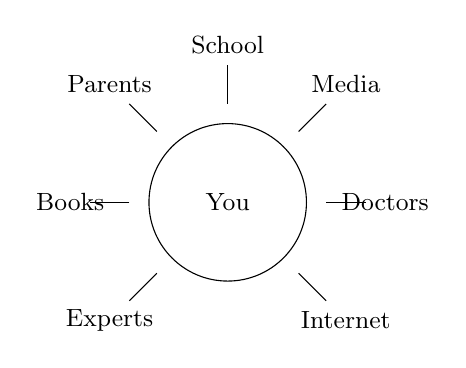
\begin{tikzpicture}[scale=0.5]
        \small
        \draw (0,0) circle (2cm);
        \node at (0,0) {You};
        \draw (0,2.5) -- (0,3.5);
        \node at (0,4) {School};
        \draw (1.8,1.8) -- (2.5,2.5);
        \node at (3,3) {Media};
        \draw (-1.8,1.8) -- (-2.5,2.5);
        \node at (-3,3) {Parents};
        \draw (2.5,0) -- (3.5,0);
        \node at (4,0) {Doctors};
        \draw (-2.5,0) -- (-3.5,0);
        \node at (-4,0) {Books};
        \draw (1.8,-1.8) -- (2.5,-2.5);
        \node at (3,-3) {Internet};
        \draw (-1.8,-1.8) -- (-2.5,-2.5);
        \node at (-3,-3) {Experts};
    \end{tikzpicture}
\end{frame}

\begin{frame}{Survival Through Trust: How Authority Arguments Keep Us Alive}
    \begin{itemize}
        \item Relying on authority is not a weakness but an evolutionary necessity for social species.
        \item Without trust in authority, we would need to personally verify every piece of knowledge we use.
        \item \textbf{Specialization} in knowledge allows society to advance far beyond what any individual could achieve.
        \item Learning from others' expertise and experience helps us avoid dangerous trial-and-error approaches.
    \end{itemize}
    
    \begin{alertblock}{Thought Experiment}
        Imagine if you had to personally verify everything you know:
        \begin{itemize}
            \item Is this mushroom poisonous?
            \item Will this bridge support my weight?
            \item Is this medical treatment effective?
            \item Is this electrical wiring safe?
        \end{itemize}
    \end{alertblock}
\end{frame}

\begin{frame}{The Doctor Said So: Everyday Examples of Authority Arguments}
    \begin{itemize}
        \item We take medication because doctors and pharmacists tell us it will help, not because we understand the biochemistry.
        \item Students accept information in textbooks because they're written by subject matter experts.
        \item We follow weather forecasts from meteorologists when planning outdoor activities.
        \item We trust engineers and architects that buildings and bridges are safely designed.
    \end{itemize}
    
    \begin{table}
        \begin{tabular}{|l|l|l|}
            \hline
            \textbf{Domain} & \textbf{Authority} & \textbf{We Trust Them On} \\
            \hline
            Health & Doctors & Medical diagnoses and treatments \\
            Law & Lawyers & Legal advice and representation \\
            Construction & Engineers & Safety of structures \\
            Education & Teachers & Subject knowledge \\
            \hline
        \end{tabular}
    \end{table}
\end{frame}

\begin{frame}{Beyond Humans: Authority in the Animal Kingdom}
    \begin{itemize}
        \item Many animal species display behaviors analogous to our reliance on authority.
        \item Young animals learn critical survival skills by observing and imitating adults.
        \item Primates have been observed deferring to more experienced members in foraging and conflict resolution.
        \item Some species have specific "teaching" behaviors where knowledge is deliberately transmitted.
    \end{itemize}
    
    \begin{example}{Honeybee Waggle Dance}
        When a forager bee discovers a food source, it communicates the location to other bees through a precise dance pattern. The other bees accept this "authority" information without independently discovering the food source first.
    \end{example}
\end{frame}

\begin{frame}{The Evolution of Authority: How We Learned to Trust Experts}
    \begin{itemize}
        \item Trust in authority likely evolved as a cognitive shortcut that conserved energy and increased survival chances.
        \item Early human societies developed specialized roles where certain individuals became experts in specific domains.
        \item \textbf{Social learning} - acquiring knowledge from others rather than through direct experience - gave humans an evolutionary advantage.
        \item As human knowledge expanded, reliance on authorities became increasingly necessary for functioning in complex societies.
    \end{itemize}
    
    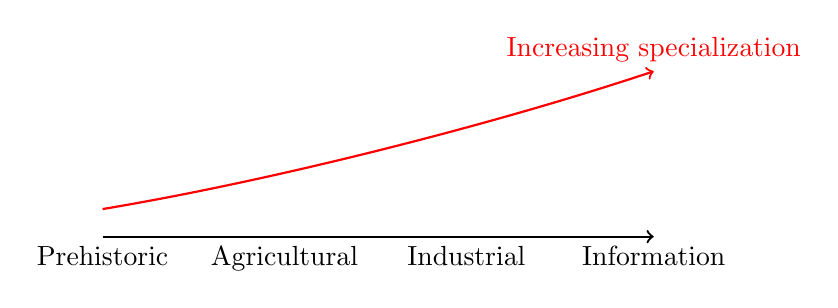
\begin{tikzpicture}[scale=0.7]
        % Timeline arrow
        \draw[thick,->] (0,0) -- (10,0);
        % Nodes for different periods
        \node[below] at (0,0) {Prehistoric};
        \node[below] at (3.3,0) {Agricultural};
        \node[below] at (6.6,0) {Industrial};
        \node[below] at (10,0) {Information};
        % Expertise complexity arrow
        \draw[thick, red, ->] (0,0.5) .. controls (3,1) and (7,2) .. (10,3);
        \node[above, red] at (10,3) {Increasing specialization};
    \end{tikzpicture}
\end{frame}

\begin{frame}{When Expertise Matters: Legitimate vs. Illegitimate Authority}
    \begin{itemize}
        \item \textbf{Legitimate authority} comes from relevant expertise, experience, or credentials in a specific domain.
        \item Authorities are most reliable when speaking within their area of expertise.
        \item \textbf{Illegitimate authority} occurs when we accept claims from people who lack genuine expertise in the relevant area.
        \item The strength of an authority argument depends on how qualified the authority actually is.
    \end{itemize}
    
    \begin{block}{Evaluating Authority Legitimacy}
        An authority's claims are more likely to be reliable when:
        \begin{itemize}
            \item They have relevant education, experience, or credentials
            \item They're speaking within their field of expertise
            \item Their views represent consensus among other experts
            \item They don't have significant conflicts of interest
        \end{itemize}
    \end{block}
\end{frame}

\begin{frame}{Inductive Reasoning: The Foundation of Authority Arguments}
    \begin{itemize}
        \item Arguments from authority are a form of \textbf{inductive reasoning}, which means they provide probable but not certain conclusions.
        \item Unlike deductive arguments that guarantee their conclusions if premises are true, inductive arguments only make their conclusions more likely.
        \item Authority arguments have degrees of strength based on the authority's qualifications and other supporting evidence.
        \item Even the strongest authority argument can be wrong in specific instances.
    \end{itemize}
    
    \begin{table}
        \scriptsize
        \centering
        \begin{tabular}{|p{5cm}|p{5cm}|}
            \hline
            \textbf{Deductive Arguments} & \textbf{Inductive Arguments} \\
            \hline
            If premises are true, conclusion must be true & If premises are true, conclusion is probably true \\
            Certainty & Probability \\
            Truth-preserving & Not truth-preserving \\
            Example: All humans are mortal. Socrates is human. Therefore, Socrates is mortal. & Example: Dr. Smith says this medication will help. Dr. Smith is a qualified doctor. Therefore, this medication will probably help. \\
            \hline
        \end{tabular}
    \end{table}
\end{frame}

\begin{frame}{The Strength Spectrum: Evaluating Authority Claims}
    \begin{itemize}
        \item Arguments from authority exist on a spectrum from very weak to very strong.
        \item The strength depends on multiple factors, including expertise relevance and consensus.
        \item \textbf{Strong authority arguments} come from well-qualified experts speaking within their domain of expertise.
        \item \textbf{Weak authority arguments} come from questionable sources or experts speaking outside their field.
    \end{itemize}
    
    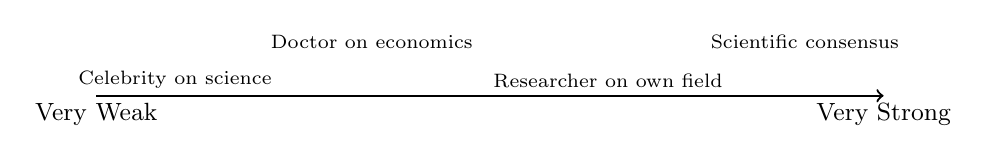
\begin{tikzpicture}
        \scriptsize
        % Create a spectrum arrow
        \draw[thick, ->] (0,0) -- (10,0);
        \node[below] at (0,0) {\small Very Weak};
        \node[below] at (10,0) {\small Very Strong};
        
        % Examples at different points
        \node[above] at (1,0) {Celebrity on science};
        \node[above] at (3.5,0.5) {Doctor on economics};
        \node[above] at (6.5,0) {Researcher on own field};
        \node[above] at (9,0.5) {Scientific consensus};
    \end{tikzpicture}
\end{frame}

\begin{frame}{Relevant Expertise: Finding the Right Authority}
    \begin{itemize}
        \item \textbf{Relevant expertise} means having knowledge and experience specifically in the domain being discussed.
        \item Expertise in one area doesn't automatically transfer to other domains, even related ones.
        \item The narrower and more specialized the field, the more important it is to find authorities with specific expertise.
        \item Practical experience can sometimes be as valuable as formal credentials, depending on the domain.
    \end{itemize}
    
    \begin{example}{Medical Specialization}
        You wouldn't ask a dermatologist about heart surgery or a cardiologist about skin conditions, even though both are medical doctors with extensive training. Their specialized expertise makes them authorities in different domains.
    \end{example}
\end{frame}

\begin{frame}{Consensus vs. Outliers: When Experts Disagree}
    \begin{itemize}
        \item \textbf{Expert consensus} occurs when a large majority of qualified authorities in a field agree on a conclusion.
        \item Consensus views are generally more reliable than the opinions of isolated outliers.
        \item However, scientific progress sometimes begins with outlier views that challenge consensus.
        \item When experts disagree, we must evaluate the strength of evidence on both sides rather than simply counting authorities.
    \end{itemize}
    
    \begin{alertblock}{Warning: Cherry-Picking Authorities}
        It's fallacious to selectively cite only those authorities who support your preferred conclusion while ignoring the broader expert consensus. This is a form of confirmation bias.
    \end{alertblock}
\end{frame}

\begin{frame}{Cognitive Shortcuts: Why Our Brains Love Authorities}
    \begin{itemize}
        \item Human brains use \textbf{cognitive heuristics} (mental shortcuts) to make decisions efficiently.
        \item The \textbf{authority heuristic} allows us to quickly process information without independently verifying everything.
        \item These shortcuts are essential for functioning in a complex world where we can't personally verify all information.
        \item However, these same shortcuts make us vulnerable to accepting false authorities or misapplying legitimate ones.
    \end{itemize}
    
    \begin{table}
        \scriptsize
        \centering
        \begin{tabular}{|p{5cm}|p{5cm}|}
            \hline
            \textbf{Benefits of Authority Heuristic} & \textbf{Risks of Authority Heuristic} \\
            \hline
            Saves cognitive resources & May accept incorrect information \\
            Enables access to specialized knowledge & Can be manipulated by false authorities \\
            Allows efficient decision-making & May dismiss valid information from non-authorities \\
            Builds on collective wisdom & Can perpetuate systemic errors \\
            \hline
        \end{tabular}
    \end{table}
\end{frame}

\begin{frame}{The Appeal to False Authority Fallacy}
    \begin{itemize}
        \item The \textbf{appeal to false authority fallacy} occurs when someone cites an authority who lacks relevant expertise on the topic.
        \item This fallacy weakens an argument because the cited authority's opinion isn't based on appropriate knowledge or experience.
        \item It often appears when complex topics are simplified or when popularity is confused with expertise.
        \item Recognizing this fallacy requires evaluating the authority's credentials relative to the specific claim.
    \end{itemize}
    
    \begin{block}{Common Forms of False Authority}
        \begin{itemize}
            \item Using celebrities to endorse scientific claims
            \item Citing someone's academic credentials in an unrelated field
            \item Appealing to historical figures on modern issues
            \item Treating personal experience as universal expertise
        \end{itemize}
    \end{block}
\end{frame}

\begin{frame}{Celebrity Endorsements: Authority Without Expertise}
    \begin{itemize}
        \item Celebrities are frequently used to promote products, ideas, or causes despite lacking relevant expertise.
        \item Their influence derives from \textbf{visibility and familiarity}, not specialized knowledge.
        \item We often confuse likability or success in one domain with authority in unrelated domains.
        \item The entertainment industry particularly relies on celebrity authority to sell products and ideas.
    \end{itemize}
    
    \begin{example}{Famous Questionable Celebrity Endorsers}
        \scriptsize
        \begin{itemize}
            \item Gwyneth Paltrow promoting alternative health products through her brand Goop.
            \item Tom Brady endorsing a controversial fitness and nutrition regimen.
            \item Jenny McCarthy advocating against vaccinations despite lacking medical expertise.
            \item Kim Kardashian promoting various beauty and diet products without scientific backing.
        \end{itemize}
    \end{example}
\end{frame}

\begin{frame}{The Halo Effect: When We Overgeneralize Expertise}
    \begin{itemize}
        \item The \textbf{halo effect} is a cognitive bias where positive impressions in one area influence our perception in unrelated areas.
        \item We tend to assume that people who excel in one domain must be competent in others as well.
        \item This bias leads us to overgeneralize authority beyond an expert's actual domain of expertise.
        \item Successful people often receive unwarranted credibility on topics unrelated to their success.
    \end{itemize}
    
    \begin{example}{Albert Einstein and Politics}
        Einstein was undoubtedly a brilliant physicist, but his opinions on politics, religion, or economics don't automatically carry the same weight as his scientific work. Yet, his quotes on these topics are often treated with special authority because of his scientific genius.
    \end{example}
\end{frame}

\begin{frame}{Transferred Authority: When Experts Step Outside Their Field}
    \begin{itemize}
        \item \textbf{Transferred authority} occurs when legitimate experts speak authoritatively outside their area of expertise.
        \item Even brilliant minds can make amateur mistakes when venturing beyond their specialization.
        \item Expertise rarely transfers completely between fields, even those that seem closely related.
        \item We should evaluate claims based on domain-specific expertise, not general intelligence or success.
    \end{itemize}
    
    \begin{alertblock}{Warning Sign}
        Be cautious when an authority figure prefaces their claim with phrases like "I'm not an expert in this, but..." or "This isn't my field, however..." while still expecting their opinion to carry weight.
    \end{alertblock}
\end{frame}

\begin{frame}{Evaluating Credentials: What Makes Someone an Expert?}
    \begin{itemize}
        \item \textbf{Expertise} typically combines formal education, practical experience, peer recognition, and a track record of contributions.
        \item Formal credentials (degrees, certifications) provide baseline knowledge but aren't always sufficient.
        \item Active participation in a field through research, publication, or practice demonstrates ongoing expertise.
        \item Recognition by other experts in the field serves as a validity check on claimed expertise.
    \end{itemize}
    
    \begin{table}
        \centering
        \begin{tabular}{|l|p{7cm}|}
            \hline
            \textbf{Component} & \textbf{Why It Matters} \\
            \hline
            Education & Provides foundational knowledge and theoretical understanding \\
            Experience & Builds practical skills and contextual understanding \\
            Peer Recognition & Validates expertise through assessment by other experts \\
            Contributions & Demonstrates ability to advance knowledge in the field \\
            \hline
        \end{tabular}
    \end{table}
\end{frame}

\begin{frame}{The Bandwagon Effect: Confusing Popularity With Authority}
    \begin{itemize}
        \item The \textbf{bandwagon effect} occurs when people believe something because many others believe it.
        \item Popularity is not the same as expertise; widely held beliefs can still be incorrect.
        \item This effect amplifies in social media environments where likes and shares can create an illusion of authority.
        \item Conformity pressure makes us more likely to accept popular views without critical evaluation.
    \end{itemize}
    
    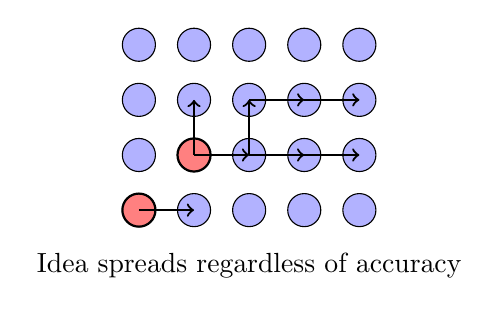
\begin{tikzpicture}[scale=0.7]
        % Draw circles representing people
        \foreach \x in {1,...,5} {
            \foreach \y in {1,...,4} {
                \fill[blue!30] (\x,\y) circle (0.3);
                \draw (\x,\y) circle (0.3);
            }
        }
        
        % Highlight a few as "originators"
        \fill[red!50] (1,1) circle (0.3);
        \draw[thick] (1,1) circle (0.3);
        \fill[red!50] (2,2) circle (0.3);
        \draw[thick] (2,2) circle (0.3);
        
        % Add arrows showing influence
        \draw[->, thick] (1,1) -- (2,1);
        \draw[->, thick] (2,2) -- (3,2);
        \draw[->, thick] (2,2) -- (2,3);
        \draw[->, thick] (3,2) -- (4,2);
        \draw[->, thick] (3,2) -- (3,3);
        \draw[->, thick] (3,3) -- (4,3);
        \draw[->, thick] (4,2) -- (5,2);
        \draw[->, thick] (4,3) -- (5,3);
        
        \node at (3,0) {Idea spreads regardless of accuracy};
    \end{tikzpicture}
\end{frame}

\begin{frame}{Bias in Authority: When Experts Have Conflicts of Interest}
    \begin{itemize}
        \item \textbf{Conflicts of interest} arise when an authority has personal, financial, or professional stakes in their claims.
        \item Even legitimate experts can have their judgment compromised by competing interests.
        \item Disclosure of conflicts is essential but doesn't automatically eliminate the potential for bias.
        \item Evaluating authority requires considering both expertise and potential motivations.
    \end{itemize}
    
    \begin{alertblock}{Red Flags for Conflicts of Interest}
        Be especially vigilant when:
        \begin{itemize}
            \item Research is funded by companies with a stake in the outcome
            \item Experts have financial relationships with affected industries
            \item Authorities stand to gain fame, status, or power from their claims
            \item Experts are advocating within highly politicized or controversial domains
        \end{itemize}
    \end{alertblock}
\end{frame}

\begin{frame}{Outdated Expertise: Authority in Rapidly Changing Fields}
    \begin{itemize}
        \item Knowledge in many fields evolves rapidly, making expertise temporary without continuous learning.
        \item \textbf{Outdated expertise} occurs when authorities rely on knowledge that has been superseded by new discoveries.
        \item The half-life of knowledge varies dramatically between fields—some change monthly, others remain stable for decades.
        \item Expert authorities must demonstrate continued engagement with current research and developments.
    \end{itemize}
    
    \begin{block}{Knowledge Half-Life by Field}
        \begin{description}
            \item[Technology] around 1-2 years (especially programming, AI)
            \item[Medicine] around 3-5 years (varies by specialty)
            \item[Physics] around 5-10 years (core theories stable, applications evolve)
            \item[History] around 10-20 years (interpretations change, facts remain)
            \item[Mathematics] around 20+ years (core principles highly stable)
        \end{description}
    \end{block}
\end{frame}

\begin{frame}{Logical Analysis: Testing Claims Beyond the Authority}
    \begin{itemize}
        \item While authority arguments are essential, they should ideally be supplemented with other forms of evidence.
        \item \textbf{Logical analysis} involves examining the internal consistency and plausibility of claims.
        \item Look for clear reasoning, appropriate evidence, and absence of logical fallacies in expert claims.
        \item The best authorities explain their reasoning rather than simply asserting conclusions.
    \end{itemize}
    
    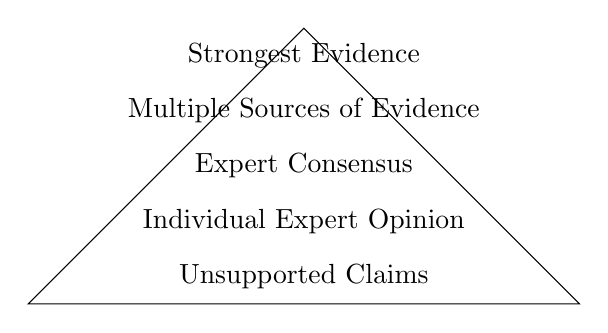
\begin{tikzpicture}[scale=0.7]
        % Draw a hierarchy of evidence diagram
        \draw (0,0) -- (5,5) -- (10,0) -- cycle;
        
        % Label the levels
        \node at (5,4.5) {Strongest Evidence};
        \node at (5,3.5) {Multiple Sources of Evidence};
        \node at (5,2.5) {Expert Consensus};
        \node at (5,1.5) {Individual Expert Opinion};
        \node at (5,0.5) {Unsupported Claims};
    \end{tikzpicture}
\end{frame}

\begin{frame}{Case Study: Climate Science and Authority}
    \begin{itemize}
        \item Climate science demonstrates the complexities of authority-based reasoning in modern scientific disputes.
        \item Scientific consensus on climate change developed through thousands of independent studies and expert analyses.
        \item The public debate often features competing claims to authority from scientists with varying credentials.
        \item This case illustrates how to distinguish between \textbf{domain-specific expertise} and general scientific credentials.
    \end{itemize}
    
    \begin{alertblock}{Key Lesson}
        The scientific consensus on climate change is based not on a single authority but on multiple lines of evidence evaluated by thousands of scientists with relevant expertise. This demonstrates how the strongest authority arguments are those where multiple qualified experts independently reach similar conclusions.
    \end{alertblock}
\end{frame}

\begin{frame}{Authority in Different Contexts: Diverse Perspectives}
    \begin{itemize}
        \item Different contexts value different types of authority and approach authority claims in distinct ways.
        \item Some situations emphasize traditional, hierarchical, or age-based authority; others prioritize credentials or demonstrated results.
        \item \textbf{Contextual factors} influence which authorities we recognize and how strongly we weigh their claims.
        \item Understanding these differences helps navigate communication about expert knowledge.
    \end{itemize}
    
    \begin{table}
        \centering
        \begin{tabular}{|l|l|}
            \hline
            \textbf{Context} & \textbf{Type of Authority Valued} \\
            \hline
            Academic & Credential-based authority \\
            Medical & Expertise-based authority \\
            Corporate & Hierarchical authority \\
            Community & Age-based and communal authority \\
            \hline
        \end{tabular}
    \end{table}
\end{frame}

\begin{frame}{Media Literacy: Spotting Authority Claims in News}
    \begin{itemize}
        \item News media frequently use authority claims to establish credibility for their reporting.
        \item \textbf{Media literacy} includes the ability to identify and evaluate the authorities cited in news stories.
        \item Anonymous sources present a special challenge, as their expertise cannot be directly evaluated.
        \item Understanding how media frames authority helps us consume news more critically.
    \end{itemize}
    
    \begin{block}{Common Media Authority Phrases}
        Pay attention to how authorities are introduced:
        \begin{itemize}
            \item "Experts say..." (Which experts? What field?)
            \item "According to sources familiar with..." (What makes them reliable?)
            \item "Studies show..." (Which studies? By whom? Peer-reviewed?)
            \item "Officials confirmed..." (Which officials? First-hand knowledge?)
        \end{itemize}
    \end{block}
\end{frame}

\begin{frame}{Advertising and Authority: Selling Products Through Expertise}
    \begin{itemize}
        \item Advertisers frequently use authority figures to enhance product credibility and persuasiveness.
        \item \textbf{White coat effect} refers to using scientific or medical imagery to suggest authority, even without actual expertise.
        \item Products often claim to be "doctor recommended" or "scientifically proven" with minimal supporting evidence.
        \item Understanding these persuasive techniques helps consumers make more informed decisions.
    \end{itemize}
    
    \begin{table}
        \centering
        \begin{tabular}{|l|p{7cm}|}
            \hline
            \textbf{Authority Technique} & \textbf{Example in Advertising} \\
            \hline
            Expert Endorsement & "9 out of 10 dentists recommend..." \\
            Scientific Imagery & Lab coats, test tubes, and charts without actual data \\
            Implied Expertise & Using technical jargon without substantive claims \\
            Institutional Authority & University or hospital logos suggesting endorsement \\
            \hline
        \end{tabular}
    \end{table}
\end{frame}

\begin{frame}{Balancing Skepticism and Trust}
    \begin{itemize}
        \item The goal is not to reject all authority but to develop \textbf{informed trust} in appropriate authorities.
        \item Healthy skepticism involves questioning claims and seeking understanding, not automatic dismissal.
        \item Over-skepticism can be as problematic as over-trust, leading to rejection of valuable expert knowledge.
        \item Finding the right balance means being open to authority claims while evaluating them critically.
    \end{itemize}
    
    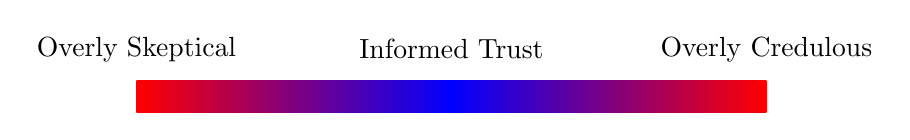
\begin{tikzpicture}[scale = .8]
        % Draw a shaded line
        \shade[left color=red, right color=red, middle color=blue] (0,0) rectangle (10,0.5);
        
        % Label the ends and middle
        \node at (0,1) {Overly Skeptical};
        \node at (10,1) {Overly Credulous};
        \node at (5,1) {Informed Trust};
    \end{tikzpicture}
\end{frame}

\begin{frame}{Exercise: Identifying Authority Arguments in Your Life}
    \begin{itemize}
        \item Authority arguments appear constantly in our daily decisions and beliefs.
        \item Becoming aware of when you're relying on authority helps develop critical thinking skills.
        \item Analyzing how you evaluate different authorities reveals potential biases in your own thinking.
        \item Practicing authority evaluation on low-stakes topics builds skills for more important decisions.
    \end{itemize}
    
    \begin{block}{Exercise Instructions}
        \scriptsize
        For one full day, keep a log of authority-based claims you encounter:
        \begin{enumerate}
            \item Record each instance where you accept something based on authority
            \item Note the type of authority (expert, traditional, institutional, etc.)
            \item Rate how critically you evaluated the claim (1-5)
            \item Identify what additional evidence would strengthen or weaken the claim
        \end{enumerate}
    \end{block}
\end{frame}

\begin{frame}{Practical Application: When to Accept Authority Claims}
    \begin{itemize}
        \item Authority arguments are more acceptable when immediate verification is impractical or impossible.
        \item Higher-stakes decisions warrant more thorough evaluation of authority claims.
        \item Look for \textbf{converging evidence} where multiple independent authorities reach similar conclusions.
        \item Be particularly cautious of authority claims that align too perfectly with your existing beliefs.
    \end{itemize}
    
    \begin{table}
        \scriptsize
        \centering
        \begin{tabular}{|p{3.5cm}|p{3.5cm}|p{3.5cm}|}
            \hline
            \textbf{Low Scrutiny Needed} & \textbf{Moderate Scrutiny Needed} & \textbf{High Scrutiny Needed} \\
            \hline
            Established scientific facts & Current medical advice & Medical treatment decisions \\
            Routine technical instructions & Financial advice & Major investments \\
            Basic historical information & Product recommendations & Political policy positions \\
            Common knowledge in a field & News from reputable sources & Claims that challenge consensus \\
            \hline
        \end{tabular}
    \end{table}
\end{frame}

\begin{frame}{Final Thoughts: Navigating a World of Authority Claims}
    \begin{itemize}
        \item Arguments from authority are neither inherently fallacious nor automatically valid.
        \item They exist on a spectrum of strength depending on the authority's qualifications and the claim's context.
        \item Developing \textbf{critical information literacy} is essential for evaluating the flood of authority claims in modern life.
        \item The most valuable skill is knowing when to trust, when to question, and how to evaluate authority claims appropriately.
    \end{itemize}
    
    \begin{alertblock}{Remember}
        We cannot personally verify every claim we encounter. Learning to properly evaluate and use arguments from authority is not just an academic exercise—it's a fundamental life skill that affects everything from your health decisions to your understanding of the world.
    \end{alertblock}
\end{frame}

\end{document}